\documentclass{article}

\usepackage[utf8]{inputenc}
\usepackage[T1]{fontenc}
\usepackage[french]{babel}
\usepackage[top=2cm,bottom=2cm,left=3cm,right=3cm]{geometry}
\usepackage{array}
\usepackage{hyperref}
\usepackage{xcolor}
\usepackage{listings}
\usepackage{fancybox}
\usepackage{tikz}
\usepackage{pgfplots}
\usepackage{tocloft}
\usepackage{graphicx}
\usepackage[raccourcis]{FAST}
\usepackage{algorithm2e}
\usepackage{circuitikz}
\usepackage{tikz-er2}
\usepackage{amsmath}
\usepackage{amssymb}
\usepackage{mathrsfs}

% Paramètres language
\lstset{basicstyle=\normalsize,
	numbers=left,
	numberstyle=\color{black}\normalsize\textbf,
	numbersep=7pt,
	backgroundcolor=\color{white},
	commentstyle=\color{black}\textit,
	keywordstyle=\color{black}\textbf,
	rulecolor=\color{black},
	stringstyle=\color{black}\textit,
	identifierstyle=\color{black},
	frame=none,
	showstringspaces=true,
}

\hypersetup{
	colorlinks=true
}

\setcounter{tocdepth}{3} % Profondeur de la table de matières
\newcommand{\vc}[1]{\overrightarrow{#1}}

\title{Valib\\-- PPE --}
\author{Luc Chabassier}

\begin{document}
\maketitle
\tableofcontents

\section{Suivit de l'utilisateur.}
Le suivit de l'utilisateur est une des premières tâches dont doit s'occuper le robot, et est l'une de ses fonctions principales. Plusieurs approches ont étés abordées, car peu d'entre elles ont aboutit.

\subsection{Ondes électromagnétiques.}
L'idée d'utiliser des ondes électromagnétiques vient d'un constat simple : tous les smartphones actuels ont des fonctionnalités Wifi et/ou bluetooth. Utiliser ces fonctionnalités pour le suivit de l'utilisateur permet d'éviter d'imposer à l'utilisateur le transport de matériel de localisation supplémentaire. De plus, les ondes électromagnétiques ont l'avantage de traverser la matière, permettant un suivit même lors d'une perte de vue du robot.

\subsubsection{Approche temporelle}
\paragraph{Principe.}
À l'aide de la durée $t$ de trajet des ondes allant du smartphone aux capteurs que nous appellerons $c_1(x_1,y_1,z_1)$, $c_2(x_2,y_2,z_2)$ et $c_3(x_3,y_3,z_3)$. Nous avons donc trois durées, $t_1$, $t_2$ et $t_3$. Comme nous connaissons la vitesse de la lumière $c=299792458m.s^{-1}$, nous pouvons déduire les distances respectives $d_1$, $d_2$ et $d_3$ entre le smartphone et les capteurs. Si nous posons le smartphone de coordonnées $S(x,y,z)$, on obtient les équations de trois sphère $C_1$, $C_2$ et $C_3$, dont nous pouvons chercher l'intersection :
\begin{enumerate}
    \item $(x-x_1)^2 + (y-y_1)^2 + (z-z_1)^2 = d_1^2$
    \item $(x-x_2)^2 + (y-y_2)^2 + (z-z_2)^2 = d_2^2$
    \item $(x-x_3)^2 + (y-y_3)^2 + (z-z_3)^2 = d_3^2$
\end{enumerate}

\paragraph{Calculs.}
Nous pouvons choisir librement le repère dans lequel nous travaillons et la position de capteurs. Afin de simplifier les calculs, nous posons le premier capteurs à l'origine $c_1(0;0;0)$, le deuxième sur l'axe x $c_2(d;0;0)$ et le troisième sur l'axe y $c_3(0;d;0)$. Nous obtenons le système suivant :
\begin{enumerate}
    \item $x^2 + y^2 + z^2 = d_1^2$
    \item $(x-d)^2 + y^2 + z^2 = d_2^2$
    \item $x^2 + (y-d)^2 + z^2 = d_3^2$
\end{enumerate}

En soustrayant l'équation 1 à la 2, on trouve :
\[2xd=d_1^2-d_2^2+d^2\]
\[x = \frac{d_1^2- d_2^2 + d^2}{2d}\]

On suppose que $\Omega(C_1 \cap C_2) > 1$.

On injecte $x$ dans l'équation 1 :
\[ \left(\frac{d_1^2-d_2^2+d^2}{2d}\right)^2 + y^2 + z^2 = d_1^2 \]
\[ y^2 + z^2 = d_1^2 - \frac{(d_1^2 - d_2^2 + d^2)^2}{4d^2} = \frac{4d_1^2d^2 - (d_1^2 - d_2^2 + d^2)^2}{4d^2} \]

C'est l'équation du cercle $(C_1 \cap C_2)$.

De plus, on a $z^2 = d_1^2-x^2-y^2$. On l'injecte dans la troisième équation :

\[ x^2 + y^2 - 2yd + d^2 + d_1^2 - x^2 - y^2 = d_3^2 \]
\[ y = -\frac{d_3^2 - d_1^2 - d^2}{2d} \]

Enfin, on a $z = \pm\sqrt{d_1^2-x^2-y^2}$.

On constate qu'il peut y avoir zéro, une ou encore deux solutions pour $z$. Dans le premier cas, on se contentera d'ignorer $z$. En effet, le robot ne se déplace que sur un plan, et donc il n'a pas besoin de connaitre la hauteur de la personne qu'il suit. Cette hauteur est uniquement utilisée pour détecter la distance entre le robot et la valise. Ceci nous permet aussi d'ignorer le cas où il y a deux solutions : qu'il soit plus haut ou plus bas, la distance sera la même, donc on choisira toujours la valeur positive de $z$. Il est de plus beaucoup plus probable que ce soit la bonne, puisque, si l'utilisateur se déplace sur un sol plat, son smartphone devrait rarement descendre en dessous des capteurs, relativement proches du sol.

\paragraph{Simulation.}
Afin de tester ces calculs, nous avons réalisé deux programmes. Le premier, qui sera à terme intégré dans le robot, utilise ces formules pour retrouver les coordonnées du smartphone par rapport au temps de trajet. Le deuxième programme, lui, génère des coordonnées aléatoires pour le smartphone, et connaissant les coordonnées des capteurs, calcule la durée du trajet de l'onde du smartphone vers les différents capteurs. Il envoie ensuite ces données au premier programme et compare les résultats avec les coordonnées initiales du smartphone.

Après avoir lancé ce test de nombreuses fois, on constate une précision très élevée, au centième de millimètre. Cette précision est bien trop élevée par rapport à nos besoins (une précision à $50cm$ serait suffisante). De plus, elle repose sur des valeur de temps quasiment exactes, precises à $10^{-13}s$. Cette précision en temps est bien supérieure à ce que nous pouvons physiquement obtenir. On constate au passage que les durées sont de l'ordre de $10^{-8}$ secondes.

\paragraph{Précision nécessaire.}
Afin de savoir de quelle précision nous avons besoin au niveau temporel, nous allons refaire des tests en arrondissant les valeurs temporelles que nous passons à notre programme, et en observant la précision obtenue.

Après avoir lancé ces tests en boucles, il ressort que pour avoir une précision de $50cm$, il faut un précision de $10^{-11}s$. Cette précision est trop élevée pour que nous puissions espérer l'atteindre. La méthode actuelle ne semble donc pas réalisable.

\subsubsection{Utilisation de l'intensité.}
\paragraph{Principe} La seconde approche s'inspire des petits robot suiveurs de lumière que l'on peut trouver un peut partout sur le net. L'idée est de mesurer l'intensité du signal qui arrive à chacun des capteurs et d'en déduire les coordonnées du smartphone. En effet, un flux d'ondes électromagnétiques suit la loi du carré inverse, c'est à dire que son intensité décroit avec le carré de la distance parcourue. Cette approche possède deux avantages principaux : \begin{enumerate}
    \item Il n'est pas nécessaire d'avoir des informations sur le smartphone : l'intégralité du traitement peut se faire sur le robot, ce qui simplifie la mise en œuvre.
    \item Si nous n'arrivons pas à trouver les formules mathématiques pour déduire les coordonnées du smartphone, nous pourrons toujours le suivre en comparant l'intensité du flux d'onde qui arrive aux capteurs.
\end{enumerate}

Nous allons centrer notre étude sur deux capteurs, afin de voir ce que nous pouvons obtenir. Nous nommons les capteurs $c_1$ et $c_2$. Nous avons les distance $d_1$ et $d_2$ entre le smartphone et ces capteurs ainsi que $I$ l'intensité initiale du flux, que nous ne connaissons pas. Les intensités que nous mesurons sur les capteurs sont $I_1=I*d_1^{-2}$ et $I_2=I*d_2^{-2}$. Afin de supprimer les $I$ (valeur inconnue), nous allons nous intéresser au rapport :
\[ \frac{I_1}{I_2} = \frac{d_2^2}{d_1^2} \Leftrightarrow k=\sqrt{\frac{I_1}{I_2}}=\frac{d_2}{d_1} \]

Afin de déterminer quel genre d'équation nous allons obtenir, nous utilisons un programme qui dessine une forme géométrique telle que $\frac{d_1}{d_2} = cte$. Après différents tests, nous conjecturons qu'il s'agit d'un cercle (voir figure \ref{circle}). Cependant, nous n'avons pas réussit à la démontrer mathématiquement, ni à trouver les formules pour extraire les coordonnées précises d'un ensemble de capteurs et de constantes.

\begin{figure}
    \begin{center}
        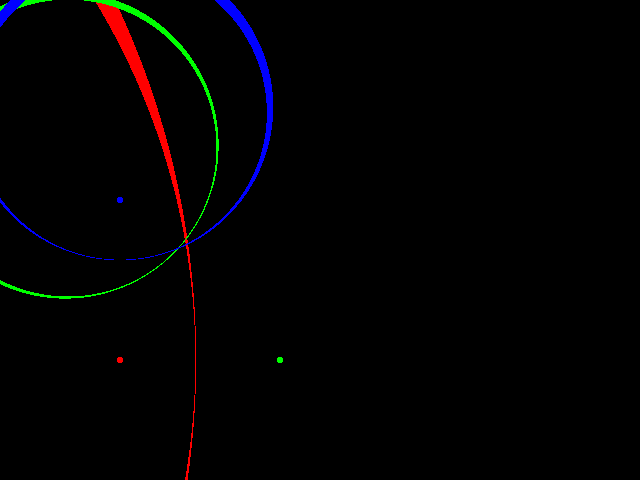
\includegraphics[width=0.75\linewidth]{rcs/circle.png}
    \end{center}
    \caption{Formes d'équation paramétrique $\frac{d_1}{d_2}=cte$.}
    \label{circle}
\end{figure}

\paragraph{Limites} Cette approche est trop difficile d'un point de vue mathématiques à mettre en œuvre, elle peut cependant permettre de suivre l'utilisateur avec des instructions simples de type gauche/droite. Mais la mise en place technique est gênée par la difficulté de trouver des capteurs d'intensité d'onde électromagnétique à exploiter.

\subsection{Utilisation d'une caméra.}
\subsubsection{Présentation.}
Cette approche vient de l'incapacité de mener à bout les deux précédentes approches et de la présence d'une unité capable de gérer des flux vidéo en temps réel pour la détection d'obstacle.

Cette approche possède de très nombreuses limites, qui l'empêche d'être une solution définitive. Nous la considérons quand même suffisante pour nos besoin, et entre dans nos capacités. Parmi ces limites, on peut citer le fait qu'il faut que l'utilisateur soit toujours dans le champ de vision de la caméra. De plus, le reconnaissance se basant sur la couleur, il faut que l'utilisateur porte un vêtement de cette couleur. Enfin, si un objet ou une personne ayant la même couleur que celle suivit entre dans le champ de vision du robot, cela risque de le perturber, et il risque de se mettre à suivre autre chose que l'utilisateur.

\subsubsection{Fonctionnement.}
Il n'y a pas de concept mathématique derrière cette approche : le robot va juste capter une image et effectuer une série de transformations dessus pour en tirer les coordonnées de l'utilisateur sur l'image, puis il verra où se il se situe par rapport à lui pour décider de la direction à prendre.

Les différentes étapes de la transformation sont : \begin{enumerate}
    \item L'image obtenue est mise dans l'espace de couleur \emph{HSV} (\emph{Hue}, \emph{Saturation}, \emph{Value}, soit teinte, saturation, valeur en français) : cet espace de couleur d'identifier une couleur en séparant cette information de l'intensité lumineuse et de la saturation, ce qui permet de retrouver la couleur même si elle est altérée par la luminosité ambiante (voir figure \ref{hsv}).
    \item L'image est ensuite binarisée suivant un modèle très simple : les trois composantes sont testées, vérifiant si elles font parties d'un encadrement préalablement déterminé. Si les trois sont validé, le pixel est mis à 1 (couleur blanche), sinon il est mis à 0 (couleur noir). Afin de déterminer ces encadrements, un programme de test a été écrit permettant de les modifier dynamiquement pour voir la meilleur combinaison possible. % TODO screenshot du programme
    \item Un algorithme de détection de contours est ensuite appliqué à l'image pour obtenir la liste des tâche blanches sur l'image. Leur aire est calculée et seule la tâche blanche avec l'aire la plus importante est gardée, ce qui permet d'éliminer les faux positifs. Si l'aire de la tâche la plus grande est trop petite, le programme considère que l'utilisateur est sorti de son champ de vision et se stoppe.
    \item Le rectangle encadrant le contour maximum est calculé, puis son centre en est déduit. Le point ainsi obtenu est considéré comme étant la position de l'utilisateur dans l'image.
        %TODO Figure présentant les différentes étapes
\end{enumerate}

\begin{figure}
    \begin{center}
        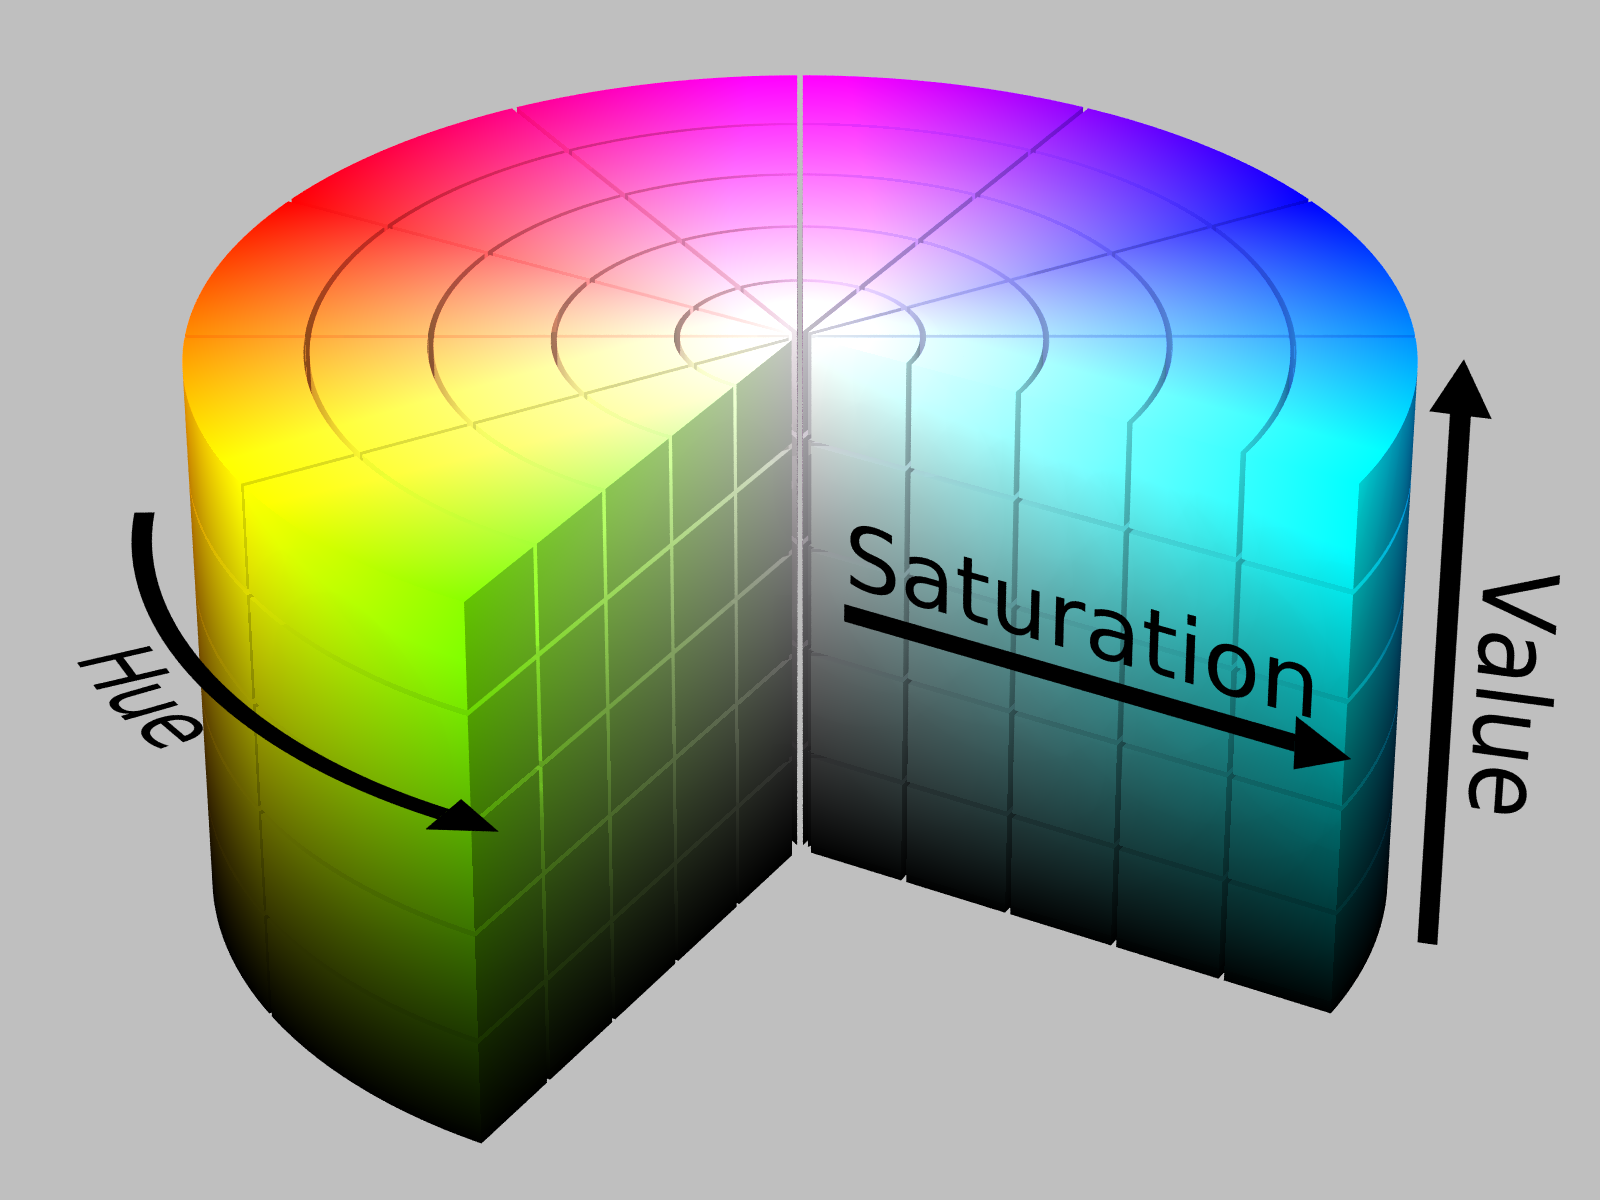
\includegraphics[width=0.75\linewidth]{rcs/hsv.png}
    \end{center}
    \caption{Présentation de l'espace de couleur \emph{HSV}.}
    \label{hsv}
\end{figure}



\section{Détection des obstacles.}
Pour l'instant, deux approches ont été explorées : la stéréo vision et une approche ABOD (\emph{Appearance Based Obstacle Detection}) dans l'espace de couleur HSV.

\subsection{Stéréo vision.}
\subsubsection{Principe.} L'idée de la stéréo vision est d'utiliser deux ou plus caméras (deux dans notre cas), et à partir des caractéristiques et positions des caméras, déduire la position dans l'espace de tout point présent sur les deux caméras. L'objectif étant d'obtenir une carte de disparité, présentant la profondeur de chaque pixel par un niveau de gris. La figure \ref{disparity} montre un exemple de carte de disparité parfaite.

\begin{figure}
    \begin{center}
        \begin{tabular}{cc}
            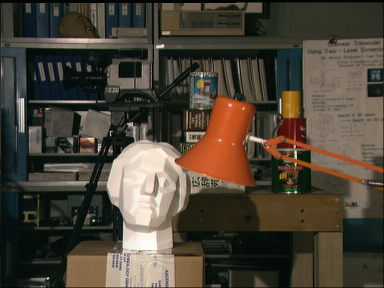
\includegraphics[width=0.4\linewidth]{rcs/tsukuba.png} & 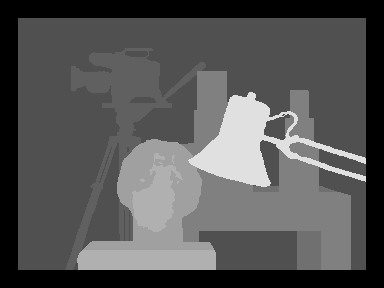
\includegraphics[width=0.4\linewidth]{rcs/tsukuba_disp.png} \\
        \end{tabular}
    \end{center}
    \caption{\emph{Tsukuba} source et sa \emph{dense disparity map}.}
    \label{disparity}
\end{figure}

\subsubsection{Calibration des caméras.}
L'étape de calibration est nécessaire pour permettre une détection de la profondeur en temps réel. Pour comprendre ce fait, il faut étudier le modèle d'une caméra : une caméra est modélisée par un point et un plan. L'image d'un point de l'espace est l'intersection entre le plan de la caméra et la droite passant par le centre de la caméra et ce point (voir figure \ref{projection}).

\begin{figure}
    \begin{center}
        \begin{tikzpicture}
            \fill (1,1) circle(0.1) node[above] {$S$};
            \fill (10,4) circle(0.1) node[above] {$P$};
            \draw [draw=black,fill=green,opacity=.3] (2,2) -- (8,0) -- (8,4) -- (2,6) -- (2,2);
            \draw [blue] (1,1) -- (10,4);
            \draw [fill=green,draw=blue] (7,3) circle(0.1) node[above, black] {$P'$};
        \end{tikzpicture}
    \end{center}
    \caption{Projection $P'$ d'un point $P$ sur une caméra de centre $S$.}
    \label{projection}
\end{figure}

Dans notre cas, avec deux caméras, nous voulons retrouver les coordonnées du point à partir de ses projections sur les deux caméras. Donc quand nous trouvons un point sur une image, il faut trouver le point correspondant sur l'autre image. Pour éviter d'avoir à chercher sur l'intégralité de l'image, nous définissons le plan homographique $H$, qui contient les centres des caméras, le point recherché et ses projection. Nous définissons ensuite les droite $(h_1)$ et $(h_2)$, intersection entre le plan homographique et les plans des caméras : voir figure \ref{homo}. Ceci nous permettrait d'optimiser la recherche des correspondances si l'on avait un méthode pour connaitre les droite homographiques associées à chaque point : il suffirait de chercher la correspondance d'un point sur la droite homographique qui lui est associé sur l'autre image.

\begin{figure}
    \begin{center}
        \begin{tikzpicture}[scale=0.8]
            \fill (1,1) circle(0.1) node[above] {$S_1$};
            \draw [draw=black,fill=green,opacity=.3] (2,2) -- (8,0) -- (8,4) -- (2,6) -- (2,2);
            \fill (19,1) circle(0.1) node[above] {$S_2$};
            \draw [draw=black,fill=green,opacity=.3] (12,0) -- (18,2) -- (18,6) -- (12,4) -- (12,0);

            \draw [red,thick] (2,3) node[above] {$(h_1)$} -- (8,3);
            \draw [red,thick] (12,3)-- (18,3) node[above] {$(h_2)$};

            \fill (10,4) circle(0.1) node[above] {$P$};
            \fill [blue,opacity=.3] (1,1) -- (19,1) -- (10,4) -- (1,1);
            \draw (10,2) node {$H$};
            \draw [blue] (1,1) -- (19,1);
            \draw [blue] (1,1) -- (10,4);
            \draw [fill=green,draw=blue] (7,3) circle(0.1) node[above, black] {$P'$};
            \draw [blue] (19,1) -- (10,4);
            \draw [fill=green,draw=blue] (13,3) circle(0.1) node[above, black] {$P''$};
        \end{tikzpicture}
    \end{center}
    \caption{Plan homographique $H$.}
    \label{homo}
\end{figure}

Pour faire ça, nous allons tirer partit d'une propriété très intéressante de ces droites : si les deux caméras sont côte à côte exactement au même niveau, les droites homographiques sont parallèles à l'axe x et alignées. La correspondance d'un point sur l'autre image a la même ordonnée, ce qui restreint les possibilités et permet d'avoir des algorithmes utilisables en temps réel.

Cependant, il est impossible de placer les caméras de manière parfaite manuellement. Nous allons donc devoir calculer des matrices qui alignerons les images. Pour ce faire, il faut placer des points dont on connait les coordonnées dans les deux images et étudier la distorsion et le décalage. Ces points sont obtenus grâce à un échiquier, dont les points sont faciles à discerner. Une fois ces matrices obtenus, il est possible de calculer la carte de disparité (\emph{disparity map}) des images des deux caméras, qui nous donnera des informations sur la profondeur.

\subsubsection{Calcul de la carte de disparité.}
Une fois les images alignées, la calcul de la carte de disparité est relativement simple puisque pris en charge par \emph{openCV}. Cependant, nous ne pouvons pas avoir une précision énorme, et il nous obtenons juste une image en niveau de gris, inexploitable en elle même. Cette carte de disparité est ensuite découpée en case, et la distance la plus proche de chaque case est calculée, afin d'être utilisé par l'algorithme de calcul de la trajectoire.

\subsubsection{Expérience} Afin de calibrer les caméras, nous utilisons une image d'échiquier que nous enregistrons sous plusieurs angle avec les deux caméras (exemple figure \ref{chess}). Nous utilisons ensuite un programme qui va détecter les coins des échiquiers dans ces images et en déduire les matrices nécessaires et qui va les stocker dans un fichier xml. Ce fichier xml sera ensuite chargé par un autre programme qui va utiliser ces matrices pour projeter les images des deux caméras, afin qu'un point sur l'une soit aligné avec le même point l'autre image. Il va ensuite utiliser l'algorithme dit de \emph{block matching} implémenté par \emph{openCV}. Il nous permet d'obtenir les cartes de disparité de chaque couple. Quelques résultats obtenus sont montrés dans la figure \ref{disp_result}. On constate que même si les résultats sont relativement bons, dans certains cas, le bruit est trop fort. Les résultats sont donc trop peu fiables pour pouvoir être exploités systématiquement. Ce problème nous a poussé à rechercher une autre approche du problème de la détection d'obstacles.

\begin{figure}
    \begin{center}
        \begin{tabular}{cc}
            \textbf{Caméra gauche} & \textbf{Caméra droite} \\
            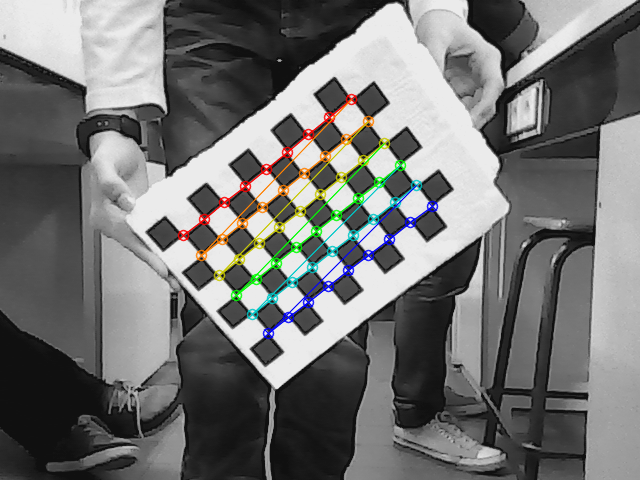
\includegraphics[width=0.4\linewidth]{rcs/chess0l.png} & 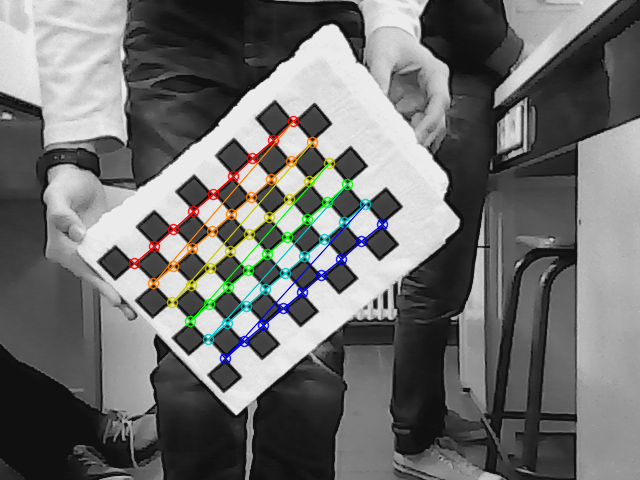
\includegraphics[width=0.4\linewidth]{rcs/chess0r.png} \\
            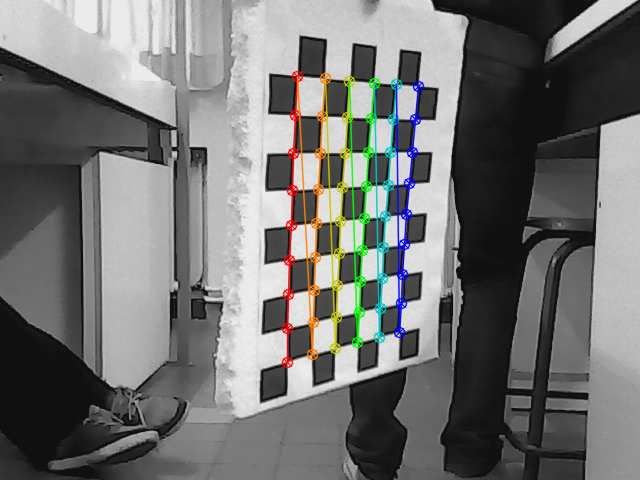
\includegraphics[width=0.4\linewidth]{rcs/chess1l.png} & 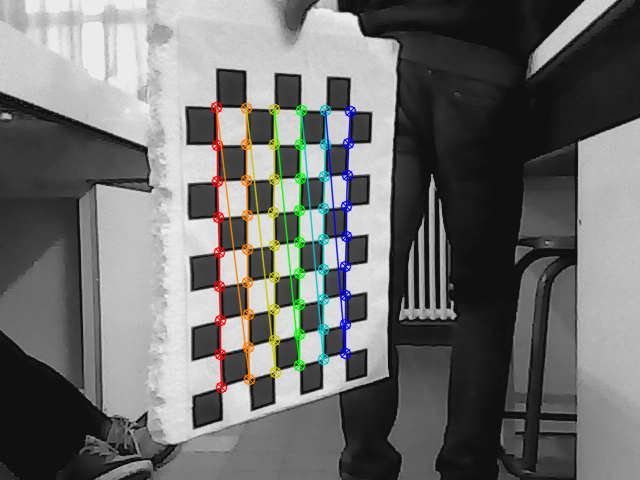
\includegraphics[width=0.4\linewidth]{rcs/chess1r.png} \\
        \end{tabular}
    \end{center}
    \caption{Exemple de couples d'images utilisés pour détecter les coins de l'échiquier.}
    \label{chess}
\end{figure}

\begin{figure}
    \begin{center}
        \begin{tabular}{ccc}
            \textbf{Caméra gauche} & \textbf{Caméra droite} & \textbf{Carte de disparité} \\
            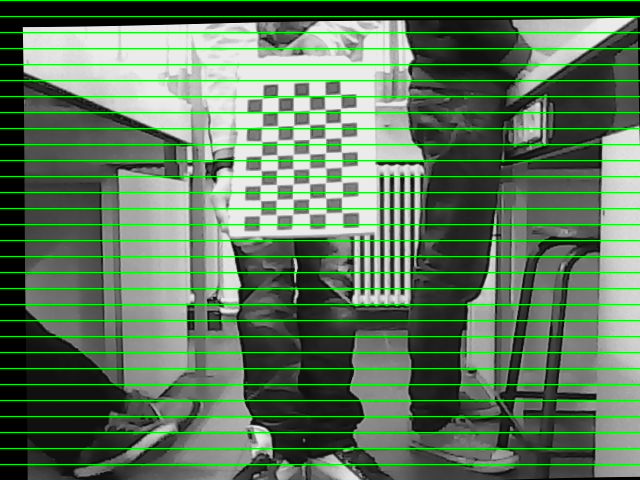
\includegraphics[width=0.3\linewidth]{rcs/rem0l.png} & 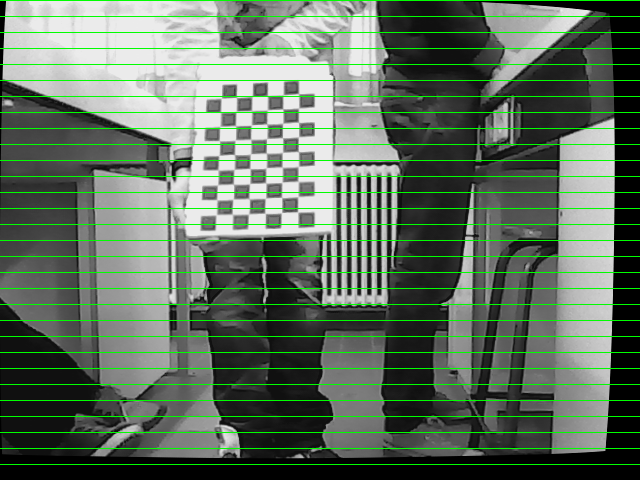
\includegraphics[width=0.3\linewidth]{rcs/rem0r.png} & 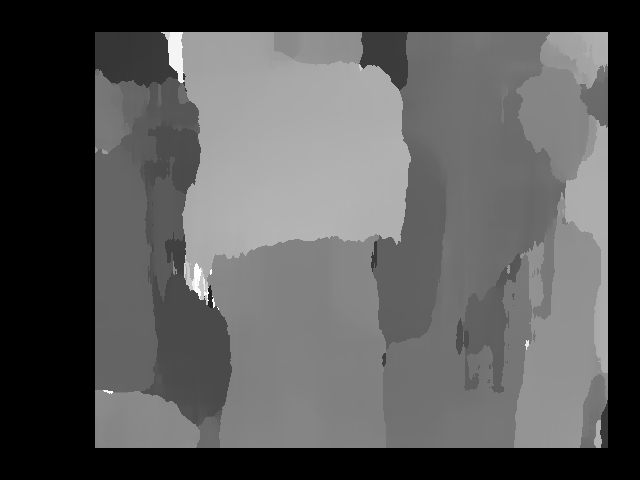
\includegraphics[width=0.3\linewidth]{rcs/disp0.png} \\
            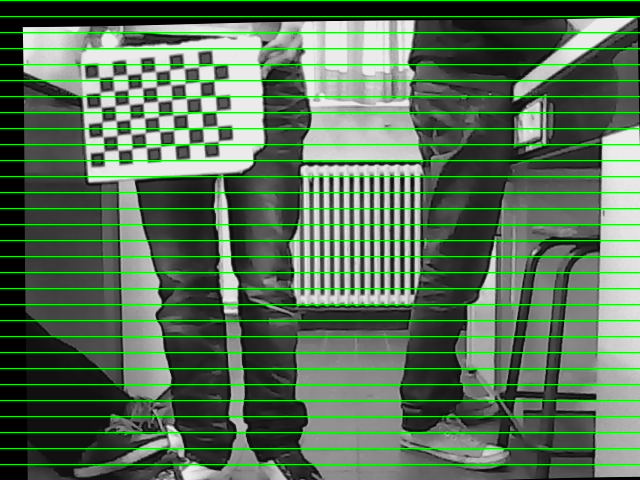
\includegraphics[width=0.3\linewidth]{rcs/rem1l.png} & 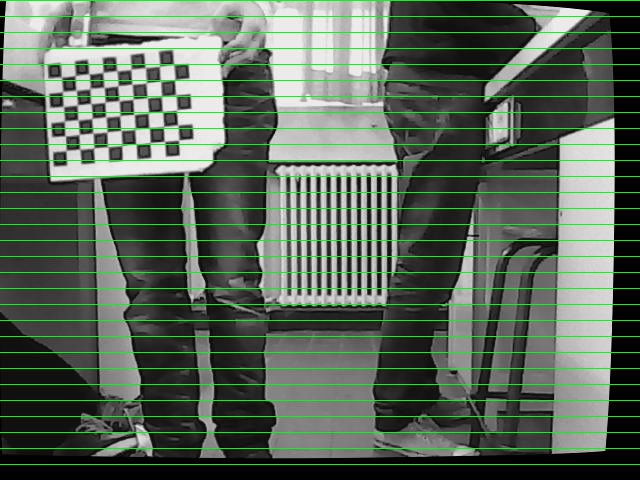
\includegraphics[width=0.3\linewidth]{rcs/rem1r.png} & 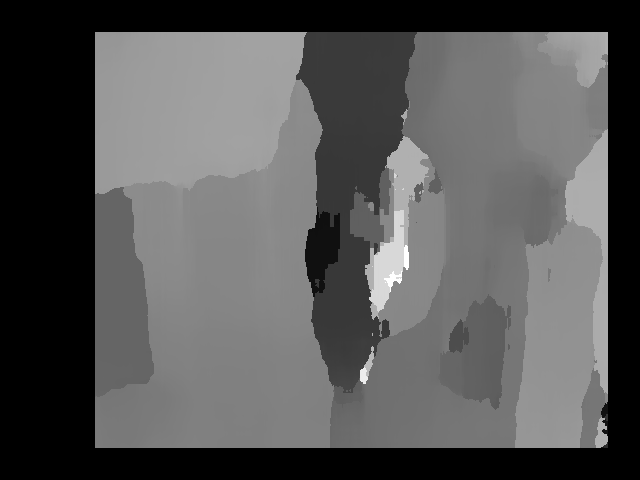
\includegraphics[width=0.3\linewidth]{rcs/disp1.png} \\
            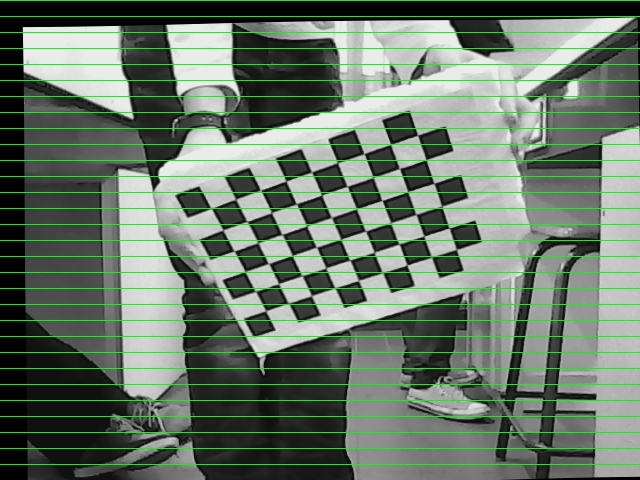
\includegraphics[width=0.3\linewidth]{rcs/rem2l.png} & 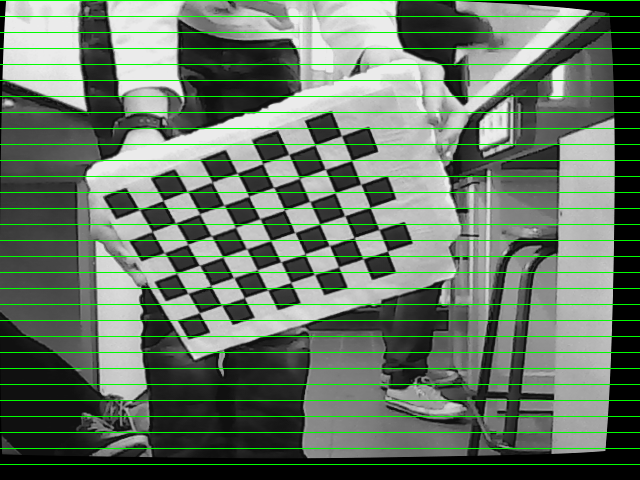
\includegraphics[width=0.3\linewidth]{rcs/rem2r.png} & 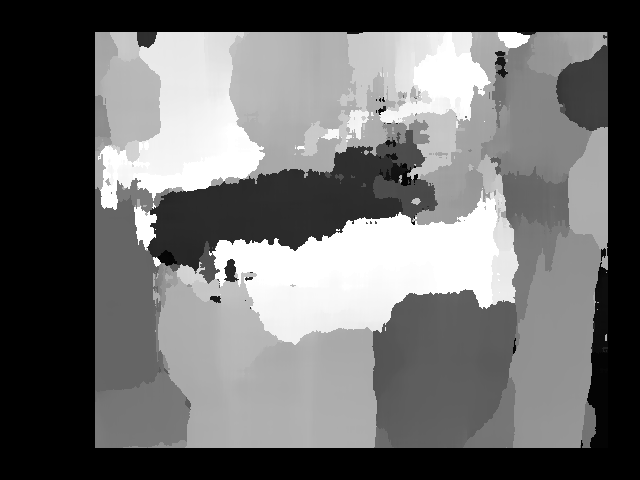
\includegraphics[width=0.3\linewidth]{rcs/disp2.png} \\
        \end{tabular}
    \end{center}
    \caption{Résultats obtenus avec la stéréo vision.}
    \label{disp_result}
\end{figure}

\subsection{Approche ABOD.}
\subsubsection{Principe} L'idée de cet algorithme est d'identifier l'apparence du sol sur le flux vidéo d'une caméra et à partir de là de différentier le sol des obstacles en se basant sur leur apparence (un exemple de résultat peut être observé sur la figure \ref{abod}). Cette algorithme possède quelques limites cependant : un obstacle comme un bord de table apparaissant dans un coin sera repéré comme un objet éloigné. En général, un obstacle \emph{volant} sera considéré comme au sol mais éloigné.

\begin{figure}
    \begin{center}
        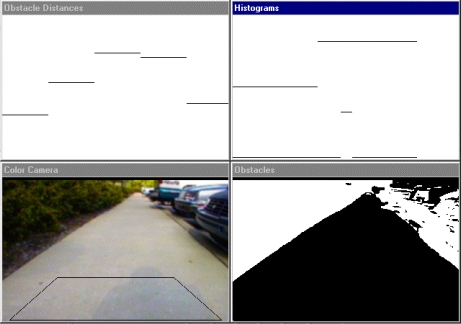
\includegraphics[width=0.8\linewidth]{rcs/abod.png}
    \end{center}
    \caption{Résultat de l'application d'un algorithme de type \emph{Appearance based obstacle detection}.}
    \label{abod}
\end{figure}

\subsubsection{Algorithme} L'idée de l'algorithme est assez simple : le sol est identifié par un histogramme, et chaque pixel de l'image est comparé à l'histogramme selon certains critères et sera classé comme appartenant au sol ou comme étant un obstacle. Afin d'affiner la détection, on décide de travailler dans l'espace de couleur \emph{HSV} et d'utiliser un procédé d'apprentissage. Lors de l'apprentissage, plusieurs images du sol seront analysées par un programme qui combinera leurs histogrammes et enregistrera l'histogramme résultant dans un fichier yaml. Ce fichier sera chargé par le robot qui l'utilisera pour différencier le sol des obstacles. Il ne peut donc fonctionner que sur un seul type de sol, ce qui n'est pas particulièrement gênant, puisqu'il est sensé fonctionner dans un seul lieu.

\subsubsection{Simulation} Afin de tester si le principe de l'algorithme est valable, on crée à l'aide du logiciel \emph{Blender} un environnement virtuel qui possède toutes les caractéristiques nécessaires : un sol unit et uniforme, plat, et des obstacles de couleur différente. Les résultats, certains exposés dans la figure \ref{abod_simu}, sont plus que satisfaisants, avec très peu de faux positifs et presque aucun faux négatifs. On observe que l'algorithme résiste bien aux tâches de lumière spéculaire, en ne les marquant pas comme obstacle.

\begin{figure}
    \begin{center}
        \begin{tabular}{|cc|}
            \hline
            \textbf{Caméra} & \textbf{Résultat} \\
            \hline & \\
            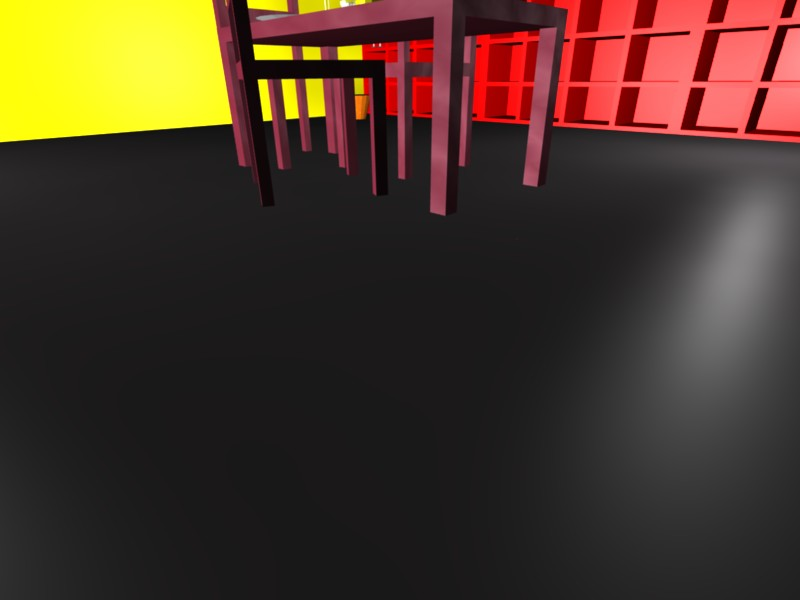
\includegraphics[width=0.4\linewidth]{rcs/abodv0s.png} & 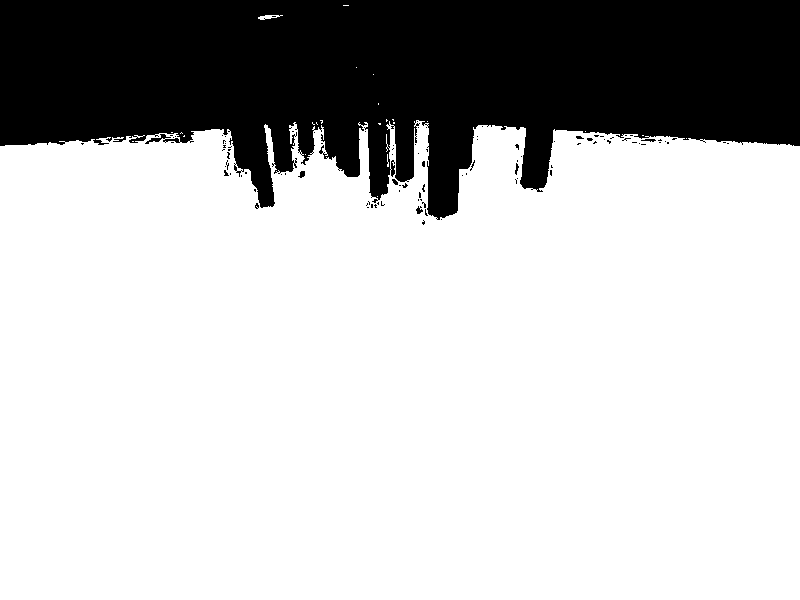
\includegraphics[width=0.4\linewidth]{rcs/abodv0r.png} \\
            \multicolumn{2}{|c|}{$1.7\%$ du sol annoncé comme obstacle et $0.1\%$ des obstacles annoncé comme sol.} \\
            \hline & \\
            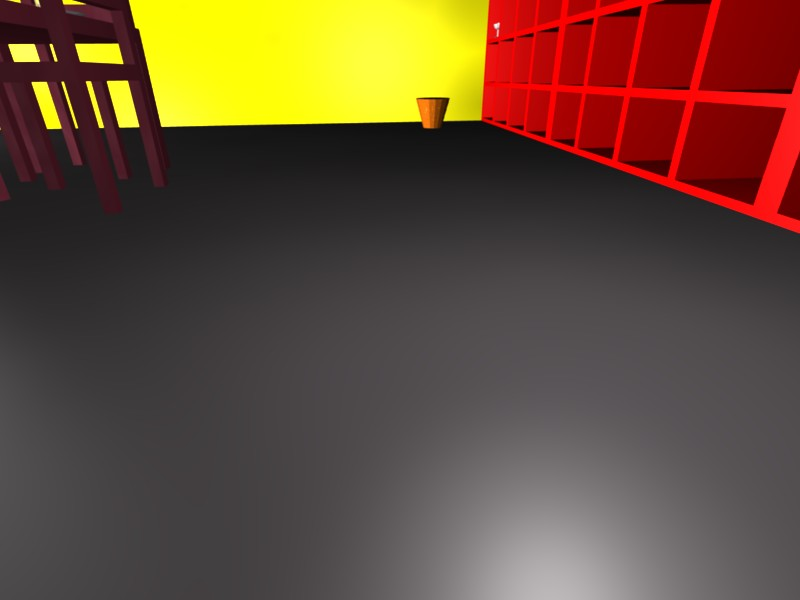
\includegraphics[width=0.4\linewidth]{rcs/abodv1s.png} & 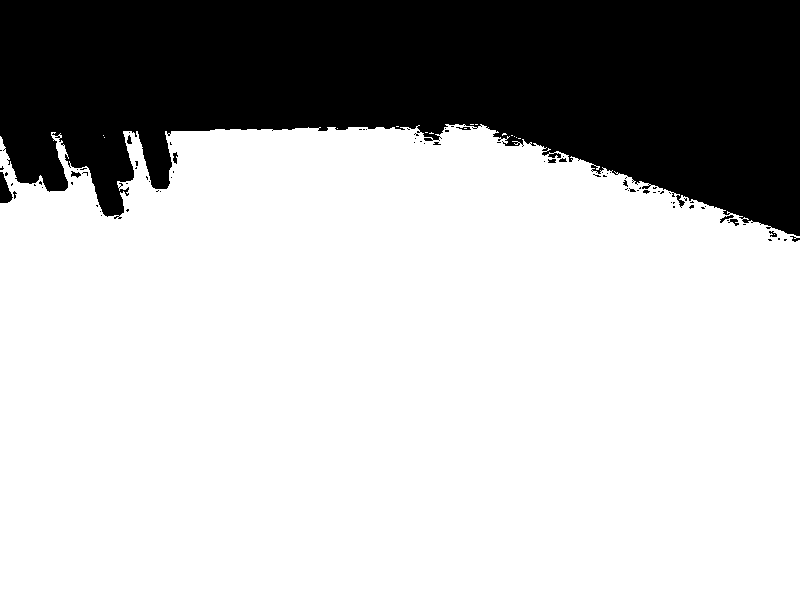
\includegraphics[width=0.4\linewidth]{rcs/abodv1r.png} \\
            \multicolumn{2}{|c|}{$1.7\%$ du sol annoncé comme obstacle et $0\%$ des obstacles annoncé comme sol.} \\
            \hline & \\
            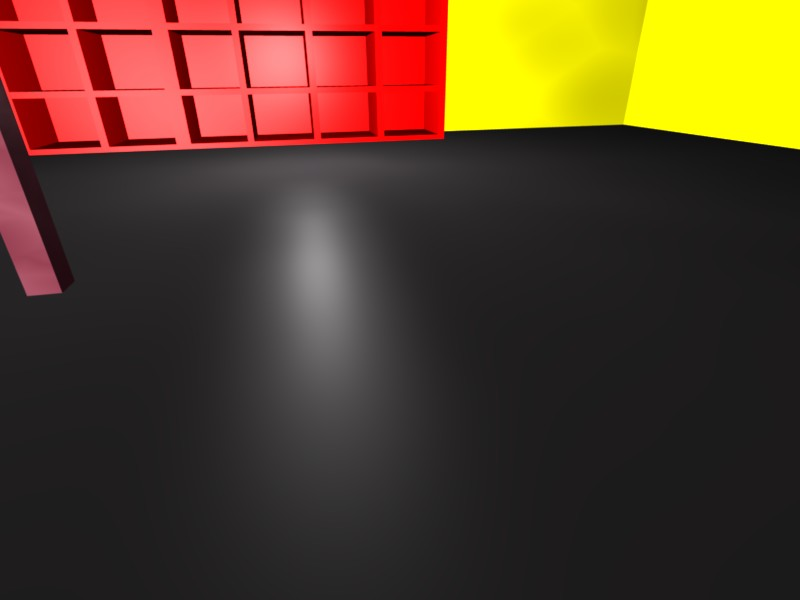
\includegraphics[width=0.4\linewidth]{rcs/abodv2s.png} & 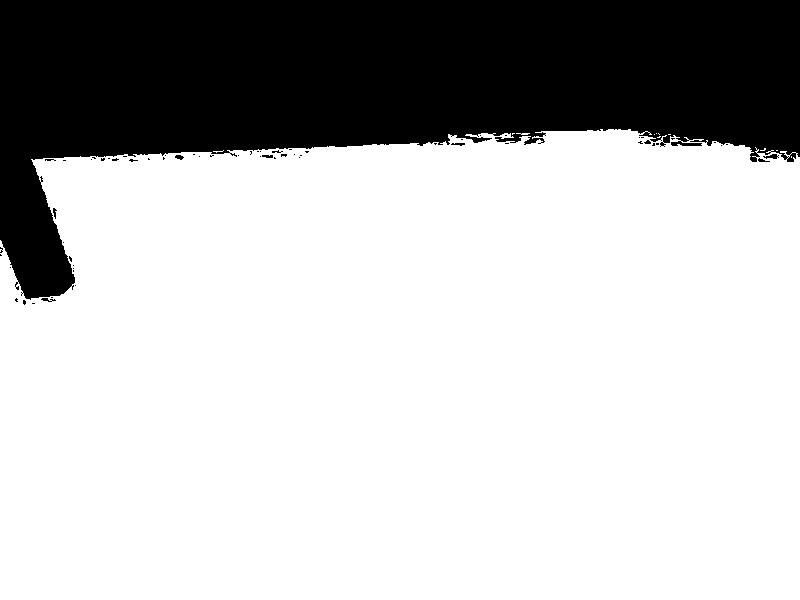
\includegraphics[width=0.4\linewidth]{rcs/abodv2r.png} \\
            \multicolumn{2}{|c|}{$0\%$ du sol annoncé comme obstacle et $1.2\%$ des obstacles annoncé comme sol.} \\
            \hline
        \end{tabular}
    \end{center}
    \caption{Résultats de l'approche \emph{ABOD} dans l'environnement virtuel.}
    \label{abod_simu}
\end{figure}

\subsubsection{Expérience.}

\subsubsection{Déduction de la distance.}
Une fois l'image binaire obtenue, il reste à en déduire la distance de chaque obstacle. Pour ce faire, l'algorithme va découper l'image horizontalement en plusieurs parties, puis pour chacune de ces parties, une détection des contours est effectuée. Le contours trop petits sont ignorés, car ils sont probablement des faux positifs. L'extrémité la plus basse des contours est calculée : c'est l'obstacle le plus proche, si l'on considère que tous les obstacles touchent le sol. Il reste à faire un lien entre la hauteur de l'obstacle sur l'image et sa distance par rapport au robot. Il faudra pour ce faire placer des obstacles à distance connue, trouver leur hauteur sur l'image, puis effectuer une regression sur ces couples de valeurs pour trouver la fonction faisant le lien.


\section{Communication.}
La communication avec l'utilisateur se basera principalement sur une communication bluetooth avec le smartphone de l'utilisateur. Peut de travail a été accomplit sur cette partie pour l'instant.

\newpage
\listoffigures
\addcontentsline{toc}{chapter}{Liste des figures.}

\end{document}

